\documentclass[tikz, border=4pt]{standalone}

% --- packages (mirror these in op-amp.meta.json "requires") ---
\usepackage{circuitikz}

% --- palette (canonical source: reference/color-palettes/color-palettes.md; light variant) ---
\definecolor{otgray}{HTML}{5A5A5A}

\begin{document}
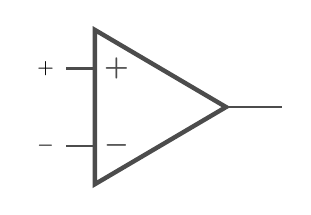
\begin{tikzpicture}
  % circuitikz's native "op amp" shape -- a real EE device symbol, so it stays
  % neutral/undyed like every other circuitikz bipole this library draws (the
  % family's domain-semantic palette colors hand-styled nodes/wires, never the
  % device glyphs themselves; see esl-crossbar-kcl's readout stage).
  \node[op amp, yscale=-1, draw=otgray!85!black, thick] (opamp) {};
  \draw (opamp.+) node[left=1pt] {\scriptsize $+$};
  \draw (opamp.-) node[left=1pt] {\scriptsize $-$};
  \draw[otgray!85!black, thick] (opamp.out) -- ++(0.35,0);
\end{tikzpicture}
\end{document}
